\chapter*{4-quadrant chopper used in railway traction CORRECTION}

\begin{enumerate}
    \item \begin{enumerate}
        \item \ 
        
        \begin{figure}[H]
            \begin{minipage}[b]{0.45\textwidth}
                \centering \underline{$\alpha < 0.5$}
            \end{minipage}
            \hfill
            \begin{minipage}[b]{0.45\textwidth}
                \centering \underline{$\alpha > 0.5$}
            \end{minipage}
            \vfill
            \begin{minipage}[b]{0.45\textwidth}
                \centering
                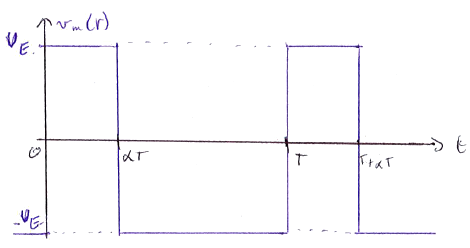
\includegraphics[width=\textwidth]{TD_H4Q/Correction/fig/H4Q_1.png}
            \end{minipage}
            \hfill
            \begin{minipage}[b]{0.45\textwidth}
                \centering
                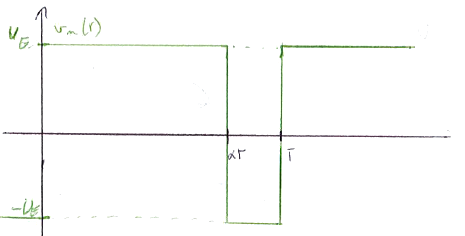
\includegraphics[width=\textwidth]{TD_H4Q/Correction/fig/H4Q_2.png}
            \end{minipage}
        \end{figure}
        \item $V_m = <v_m(t)> = \alpha U_E  - (1-\alpha) U_E  = U_E (2\alpha - 1)$
    \end{enumerate}
    \item \begin{enumerate}
        \item $U_m = (2\alpha_1-1)U_E$
        
        $V_{DC} I_E = U_m I_m \Rightarrow I_E = (2\alpha_1-1)I_m$
        \item Be carefull in this part, $C_v = -382 \text{ Nm}$ because the train is going uphill so torque is negative.
        
        $v_m(t) = R i_m(t) + L \frac{di_m(t)}{dt} + E$
        
        $V_m = <v_m(t)> = R <i_m(t)> + L <\frac{di_m(t)}{dt}> + <E>$
        \begin{itemize}
            \item $<E> = 0$ because $\Omega = 0$
            \item $<\frac{di_m(t)}{dt}> = 0 $ because $i_m(t)$ is periodic
        \end{itemize}
        \begin{equation}
            \Rightarrow V_m = (2\alpha -1) U_E = R I_m
        \end{equation}
        $J \dfrac{d\Omega}{dt} = C_m + C_v = k_\Phi i_m + C_v \Rightarrow I_M = -\dfrac{C_v}{k_\Phi}$

        (1.1) $\Rightarrow V_m = - R \dfrac{C_v}{k_\Phi} \Rightarrow \alpha_{10} = \left(1 + \dfrac{- C_v R}{k_\Phi U_E} \right) \dfrac{1}{2} \approx 0.503$

        $I_{E0} = (2\alpha_{10} - 1) I_m = (2 \alpha_{10} - 1) \dfrac{-C_v}{k_\Phi} = \dfrac{R C_v^2}{k_\Phi^2 U_E} \approx 0.33 \text{ A}$
        
        \item 
        \begin{enumerate}
            \item No resistive torque : $C_v = 0$
        
            $J \dfrac{d\Omega}{dt} = C_m + C_v = k_\Phi I_m \Rightarrow I_m = \dfrac{J}{k_\Phi} \dfrac{d\Omega}{dt} = 130 \text{ A}$

        
            \item $V_m = (2\alpha -1) U_E = R I_m + L \dfrac{di_m}{dt} + E$
            \begin{itemize}
                \item $E = K_\Phi \Omega = k_\Phi \dfrac{d\Omega}{dt} t$ because $\dfrac{d\Omega}{dt} = constant$ and ($\Omega (t=0)=0$)
                \item $\dfrac{di_m}{dt} = 0$ because $i_m = constant$ 
            \end{itemize}
            $(2\alpha -1) U_E = R I_m + k_\Phi \left(\dfrac{d\Omega}{dt}\right) t$

            $\Rightarrow \alpha (t) = \dfrac{1}{2}\left(\dfrac{R I_m}{U_E} + \dfrac{k_\Phi}{U_E} \left(\dfrac{d\Omega}{dt}\right) t + 1\right)$

            \item $\left(\dfrac{d\Omega}{dt}\right) \Delta t_a = \Omega_n \Rightarrow \Delta t_a = \dfrac{\Omega_n}{\left(\dfrac{d\Omega}{dt}\right)} = 31 \text{ s}$
        \end{enumerate}
        \item Be carefull in this part, $C_v = 382 \text{ Nm}$ because the train is going downhill so torque is positive.
        
        $J \dfrac{d\Omega}{dt} = C_m + C_v = k_\Phi i_m + C_v$

        And $\dfrac{d\Omega}{dt} = 0$ because $\Omega = constant \Rightarrow i_m = \dfrac{-C_v}{k_\Phi} = -50 \text{ A}$

        $U_E I_{Ed} = V_m I_m \Rightarrow I_{Ed}= \dfrac{V_m I_m}{U_E} = \dfrac{R I_m^2 + k_\Phi \Omega I_m}{U_E} = -39.7 \text{ A}$

        \item \begin{enumerate}
            \item $J \dfrac{d\Omega}{dt} = C_m + C_v = k_\Phi i_m + C_v$
            
            $I_m = - I_max$. The current is negative to break.

            $J \dfrac{d\Omega}{dt} = - k_\Phi I_{max} + C_v = constant \Rightarrow \Omega = \dfrac{C_v - k_\Phi I_{max}}{J} t + \Omega_n$

            \begin{figure}[H]
                \centering
                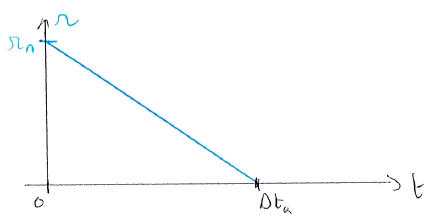
\includegraphics[width=0.6\linewidth]{TD_H4Q/Correction/fig/H4Q_Omega.png}
            \end{figure}
            \item $\Omega (t=\Delta t_a)= 0 \Rightarrow \dfrac{C_v - k_\Phi I_{max}}{J} \Delta t_a = - \Omega_n$ 
            
            $\Rightarrow \Delta t_a = \dfrac{\Omega_n J}{k_\Phi I_{max} - C_v} = 21 \text{ s}$

            \item $V_m = (2\alpha -1) U_E = R I_m + E = - R I_{max} + k_\Phi \Omega$
            
            $\Rightarrow \alpha = \dfrac{1}{2} + \dfrac{k_\Phi \Omega - R I_{max}}{2 U_E}$

            \begin{itemize}
                \item Strat breaking : $\Omega = \Omega_n \Rightarrow \alpha = 0.88$
                \item Before stop : $\Omega = 0 \Rightarrow \alpha = 0.48$
            \end{itemize}

            \item \ 
            
            $\begin{aligned}
                E_C &= \int_{0}^{\Delta t_a} -V_m I_m dt = \int_{0}^{\Delta t_a} \left(-R I_{max}^2 + k_\Phi \Omega I_{max} \right) dt \\
                &= -R I_{max}^2 \Delta t_a + \int_{0}^{\Delta t_a} k_\Phi I_{max} \left(\dfrac{C_v - k_\Phi I_{max}}{J} t + \Omega_n \right) dt \\
                & \cdots \\
                &= \dfrac{\Omega_n J}{k_\Phi I_{max} - C_v} \left( \dfrac{k_\Phi I_{max} \Omega_n}{2} - R I_{max}^2 \right) = 2.8 \text{ MJ}
            \end{aligned}$
        \end{enumerate}

        \item \ 
        
        \begin{figure}[H]
            \centering
            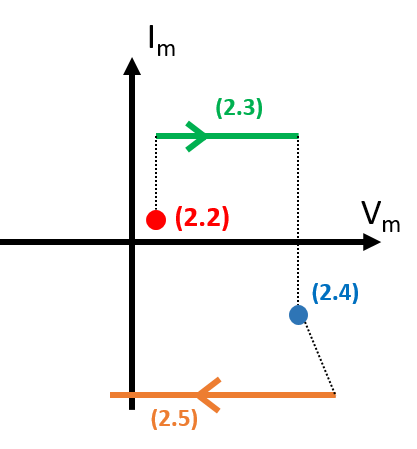
\includegraphics[width=0.6\linewidth]{TD_H4Q/Correction/fig/H4Q_quadrant.png}
        \end{figure}

        
    \end{enumerate}

\end{enumerate}